\label{sec:intro}

Reinforcement Learning (RL) research has created effective methods for training \textit{specialist} decision-making agents that maximize one objective in a single environment through trial-and-error \cite{badia2020agent57, berner2019dota, mnih2015human, silver2018general, vinyals2019grandmaster}. New efforts are shifting towards developing \textit{generalist} agents that can adapt to a variety of environments that require long-term memory and reasoning under uncertainty \cite{kirk2022survey, fan2022minedojo, team2023human, reed2022generalist}. One of the most promising approaches to generalist RL is a family of techniques that leverage sequence models to actively adapt to new situations by learning from experience at test-time. These ``in-context'' agents use memory to recall information from previous timesteps and update their understanding of the current environment \cite{wang2016learning, duan2016rl}. In-context RL's advantage is its simplicity: it reduces partial observability, generalization, and meta-learning to a single problem in which agents equipped with memory train in a collection of related environments \cite{beck2023survey, zintgraf2022fast, ghosh2021generalization}. The ability to explore, identify, and adapt to new environments arises implicitly as agents learn to maximize returns in deployments that may span multiple trials \cite{zintgraf2022fast, ortega2019meta, botvinick2019reinforcement}. 

Effective in-context agents need to be able to scale across two axes: 1) the length of their planning horizon, and 2) the length of their effective memory. The earliest versions of this framework \cite{wang2016learning, duan2016rl, stadie2018some} use recurrent networks and on-policy learning updates that do not scale well across either axis. Transformers \cite{vaswani2017attention} improve memory by removing the need to selectively write information many timesteps in advance and turning recall into a retrieval problem \cite{rae2020transformers}. Efforts to replace recurrent policies with Transformers were successful \cite{melo2022transformers, mishra2017simple}, but long-term adaptation remained challenging, and the in-context approach was relegated to an unstable baseline for other meta-RL methods \cite{beck2023survey}. However, it has been shown that pure in-context RL with recurrent networks can be a competitive baseline when the original on-policy gradient updates are replaced by techniques from a long line of work in stable off-policy RL \cite{ni2022recurrent, fakoor2019meta}. A clear next step is to reintroduce the memory benefits of Transformers. Unfortunately, training Transformers over long sequences with off-policy RL combines two of the most implementation-dependent areas in the field, and many of the established best practices do not scale (Section \ref{sec:background}). The difficulty of this challenge is perhaps best highlighted by the fact that many popular applications of Transformers in off-policy (or offline) RL devise ways to avoid RL altogether and reformulate the problem as supervised learning \cite{chen2021decision, lee2022multi, janner2021reinforcement, zheng2022online, laskin2022context, shi2023cross}.

Our work introduces AMAGO (\underline{A}daptive \underline{M}emory \underline{A}gent for achieving \underline{GO}als) --- a new learning algorithm that makes two important contributions to in-context RL. First, we redesign the off-policy actor-critic update from scratch to support long-sequence Transformers that learn from entire rollouts in parallel (Figure \ref{fig:amago}). AMAGO breaks off-policy in-context RL's biggest bottlenecks by enabling memory lengths, model sizes, and planning horizons that were previously impractical or unstable. Our agent is open-source\footnote{Code is available here: \url{https://ut-austin-rpl.github.io/amago/}} and specifically designed to be efficient, stable, and applicable to new environments with little tuning. We empirically demonstrate its power and flexibility in existing meta-RL and memory benchmarks, including state-of-the-art results in the POPGym suite \cite{morad2023popgym}, where Transformers' recall dramatically improves performance. Our second contribution takes in-context RL in a new direction with fresh benchmarks. AMAGO's use of off-policy data --- as well as its focus on long horizons and sparse rewards ---  makes it uniquely capable of extending the in-context RL framework to goal-conditioned problems \cite{kaelbling1993learning, pong2021goal} with hard exploration. We add a new hindsight relabeling scheme for \textit{multi-step} goals that generates effective exploration plans in multi-task domains. AMAGO can then learn to complete many possible instructions while using its memory to adapt to unfamiliar environments. We first study AMAGO in two new benchmarks in this area before applying it to instruction-following tasks in the procedurally generated worlds of Crafter \cite{hafner2021benchmarking}.

\begin{figure}
    \centering
    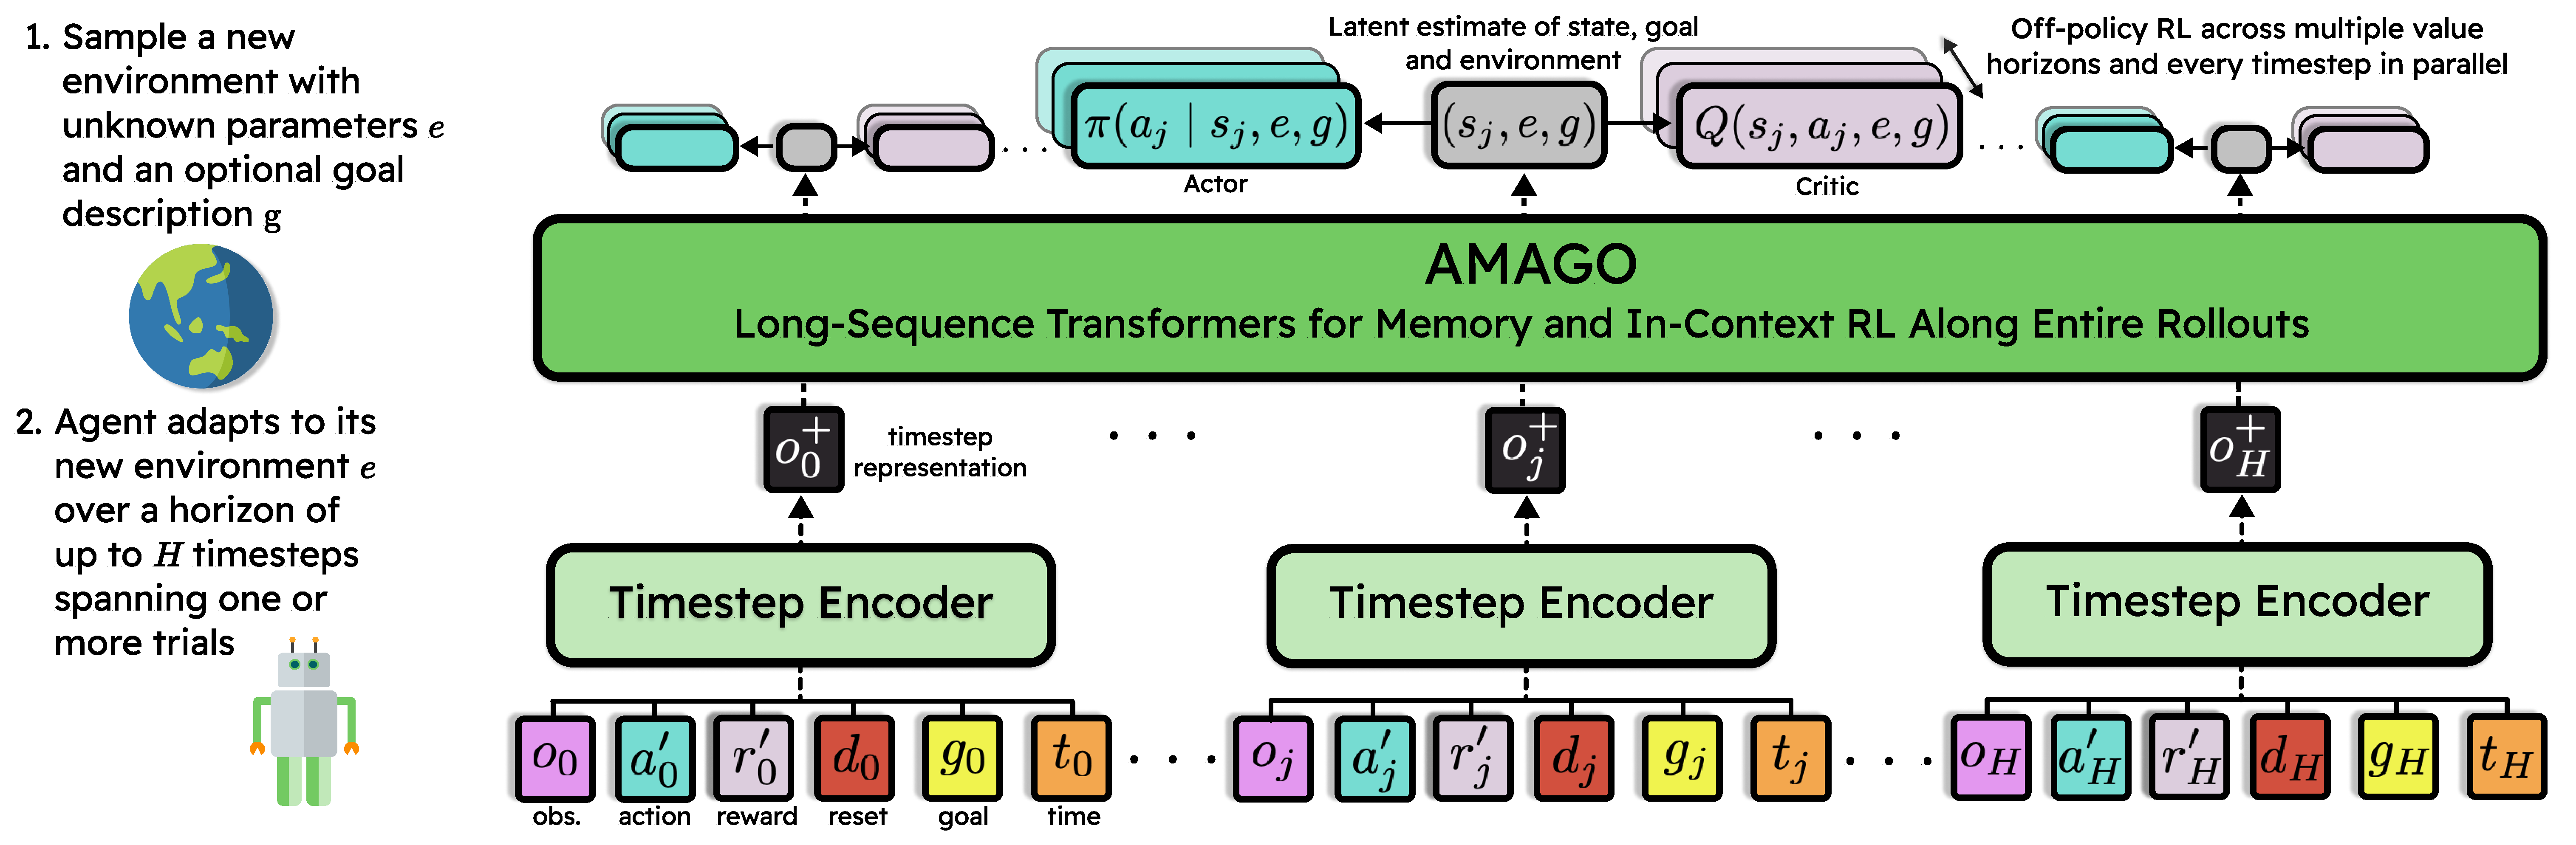
\includegraphics[width=\textwidth]{figs/fig1_iclr_e_notation.pdf}
    \caption{In-context RL techniques solve memory and meta-learning problems by using sequence models to infer the identity of unknown environments from test-time experience. AMAGO addresses core technical challenges to unify the performance of end-to-end off-policy RL with long-sequence Transformers in order to push memory and adaptation to new limits.}
    \label{fig:amago}
\end{figure}